% Template for BiDS'19 papers; to be used with:
%          spconf.sty  - LaTeX style file, and
% --------------------------------------------------------------------------
\documentclass{article}
\usepackage{spconf,amsmath,epsfig}

\providecommand{\doi}[1]{doi: {\footnotesize \href{http://dx.doi.org/#1}{\path{#1}}}}

\usepackage[pdftex=true,breaklinks=true,hidelinks=true,colorlinks=true,citecolor=blue]{hyperref}

\usepackage[square,numbers]{natbib}
\renewcommand{\bibsection}{\section*{\normalsize\hspace*{\fill}REFERENCES\hspace*{\fill}}}


% Example definitions.
% --------------------
\def\x{{\mathbf x}}
\def\L{{\cal L}}

% Title.
% ------
\title{The Pangeo Big Data Ecosystem and its use at CNES}
%
% Single address.
% ---------------
\name{Guillaume Eynard-Bontemps$^1$, Ryan Abernathey$^2$, Joseph Hamman$^3$, Aurelien Ponte$^4$}%\thanks{Thanks to XYZ agency for funding.}}
\address{$^1$Centre National d'Etudes Spatiales (CNES), Toulouse, France,\\
$^2$Columbia University / Lamont Doherty Earth Observatory, New-York, USA,\\
$^3$National Center for Atmospheric Research (NCAR), Boulder, USA,\\
$^4$Ifremer, Univ. Brest, CNRS, IRD,  Laboratoire d’Océanographie Physique et Spatiale (LOPS), IUEM, Brest 29280, France}
%
% For example:
% ------------
%\address{School\\
%	Department\\
%	Address}
%
% Two addresses (uncomment and modify for two-address case).
% ----------------------------------------------------------
%\twoauthors
%  {A. Author-one, B. Author-two\sthanks{Thanks to XYZ agency for funding.}}
%	{School A-B\\
%	Department A-B\\
%	Address A-B}
%  {C. Author-three, D. Author-four\sthanks{The fourth author performed the work
%	while at ...}}
%	{School C-D\\
%	Department C-D\\
%	Address C-D}
%
\begin{document}
%\ninept
%
\maketitle
%
\begin{abstract}
Pangeo\cite{b1} is a community driven effort for open-source big data initially
focused on the Earth System Sciences.  Its primary goal is to enable scientists
in analyzing peta-scale datasets both on classical high-performacnce computing
(HPC) and on public cloud infrastructure.  In only a few years, Pangeo has
grown into a very active community collaborating on the development of
open-source analysis tools for ocean, atmosphere and climate science, and
beyond.  It provides a set of example deployments based on open-source
Scientific Python packages like Jupyter, Dask, and xarray that not only serve as
working environments for actual scientific work, but also bring together
developers with users and their actual use-cases.

In this paper, we first describe Pangeo: its motivation, community, the
underlying technology stack and associated deployments, the different
applications and the ongoing work. We then present its impact on the work of
scientists from CNES: the context, an HPC deployment, and several use cases.
We will conclude with a future outlook for Pangeo in this agency and beyond.
\end{abstract}
%
\begin{keywords}
Pangeo, Dask, Jupyter, HPC, Cloud, Big Data, Analysis, Open Source
\end{keywords}
%
\section{Pangeo}
\label{sec:pangeo}

\subsection{Motivations, mission and goals}
\label{ssec:motivations}

The geoscience community is facing several building crises:

\begin{itemize}
\item Big Data: datasets are growing exponentially (see \ref{nasa_cloud_growth}) and legacy software tools for scientific analysis cannot handle them. This is a major technological obstacle to scientific progress.
\item Technology Gap: a growing gap between the technological sophistication of industry solutions (high) and scientific software (low).
\item Reproducibility: a fragmentation of software tools and environments renders most geoscience research effectively unreproducible and prone to failure.
\end{itemize}

\begin{figure}
  \centering
  \includegraphics[width=\columnwidth]{EOSDIS_archive_growth_updated_resize.jpg}
  \caption{\label{nasa_cloud_growth} Projected NASA EOS Cloud storage\cite{b2}.}
\end{figure}


Pangeo's core mission is to cultivate a collaborative environment in which the
next generation of open-source analysis tools for ocean, atmosphere, climate and
eventually other sciences can be developed, distributed, and sustained. These
tools must be scalable in order to meet the current and future challenges of big
data, and these solutions should leverage the existing expertise both inside and
outside of the geoscience community.

To accomplish this mission, Pangeo collaborators have identified three specific
goals.
\begin{itemize}
\item Foster collaboration around the open source Scientific Python ecosystem for the oceanographic, atmospheric, terrestrial, and climate science.
\item Support the development with domain-specific geoscience packages.
\item Improve scalability of these tools to handle petabyte-scale datasets on HPC and on cloud computing platforms.
\end{itemize}

\subsection{Community}
\label{ssec:community}

Rather than being controlled by a single organization, Pangeo is a
community-driven project, in the model of successful open-source software like
Linux, Python, and Jupyter.  In this spirit, all Pangeo discussions and products
occur on GitHub\cite{b3}, where anyone can easily get involved in the community.
As of today, Pangeo spans a list of people from different governmental agencies,
universities, or private companies, and from different countries (the USA, the
UK, France, Austalia to name a few).  By making the collaboration as broad as
possible, Pangeo successfully leverages shared expertise to accomplish things no
institution could alone.


\subsection{Technology stack}
\label{ssec:techstack}

Pangeo software ecosystem fits directly in the Scientific Python stack, involving well known packages such as Numpy, Pandas, or Sickit-learn.

%\begin{figure}
%  \centering
%  \includegraphics[width=\columnwidth]{pangeo_python_stack.png}
%  \caption{\label{scipy_stack} Pangeo Scientific Python ecosystem.}
%\end{figure}

Three Python software projects are at the core of Pangeo:
\begin{itemize}
\item Jupyter: Jupyter notebooks, Jupyter Lab, and JupyterHub enable interactive computing and analysis from a web browser and multiple user support. They are quickly becoming the standard open-source format for interactive computing in Python, as well as other languages such as Julia and R.
\item Dask is a library for parallel computing that coordinates with Python’s existing scientific software ecosystem, including libraries cited above. In many cases, it offers users the ability to take existing workflows and quickly scale them to much larger applications. Dask-distributed is an extension of Dask that facilitates parallel execution across many computers.
\item Xarray is the interface for working with big datasets: it offers a Pandas like API for dealing with labelled n-dimensionnal arrays with a self-describing scientific data capability and strong backends to standard and upcoming community data file formats and access (e.g. netCDF, GeoTIFFs, OPeNDAP).
\end{itemize}

The GitHub community offers online documentation, scripts and other tools to link them together in order to deploy a Pangeo platform (see \ref{pangeo_stack}) and put the software stack on HPC systems or in the public cloud. The main elements allowing to build and use the platforms along the core libraries are first a set of scripts and documentation that allows automatically creating the necessary cloud infrastructure. Currently available for Google Cloud Engine (GCE), and work is underway for Amazon Web Services (AWS) compatibility. Terraform software and CI/CD tooling are also under active development and offer the potential for automating these tasks.

Modules to automatically deploy distributed clusters in various infrastructures are being developed: dask-kubernetes for Kubernetes clusters and thus the public cloud, dask-jobqueue\cite{b4} for HPC systems using scheduler such as Slurm, PBS Pro or LSF, and dask-yarn for YARN clusters (i.e. Hadoop).

\begin{figure}
  \centering
  \includegraphics[width=\columnwidth]{pangeo_stack.png}
  \caption{\label{pangeo_stack} Pangeo platform main components.}
\end{figure}

\subsection{Applications}
\label{ssec:applications}

Pangeo's first scientific domain is earth sciences: particularly the domains of oceanographic, terrestrial, atmospheric, and climate sciences. There are already many applications documented in these fields. Some real science use cases can be found online\cite{b5}; these examples, along with their data, can be directly executed from a web browser. We can for example cite \textit{Sea Surface Altimetry Data Analysis} that explore the increase of global mean sea level over 20 years of data, or also \textit{US Precipitation and Temperature Analysis} that explore meteorological gridded ensemble precipitation and temperature estimates over the contiguous United States.

Other scientific domains have developed an interest in the Pangeo approach, including:
\begin{itemize}
\item Satellite imagery analysis: a recent blog post\cite{b6} explains how to use Pangeo for processing and analysing in real time Landsat imagery. NASA has decided to fund Pangeo initiative for applying the ecosystem on remote sensing datasets that are being pushed on AWS.
\item Astronomy: several scientists are already using the web platform to explore Gaia DR2 data on GCE.
\item Neuroscience: there is some on-going work to use Pangeo for analysis on human brain or electrophysiological datasets.
\end{itemize}

Such applications are most effective when deployed on cloud-optimized datasets. This means that data must be accessible in a cloud or distributed storage friendly format, like Zarr for multi-dimensional data, Cloud optimized Geotiff for satellite imagery, or Parquet for tabular data. See \cite{b7} for more details on this crucial point. Formats like NetCDF or CSV files are not adapted or optimized for use at scale.

\subsection{Ongoing work}
\label{ssec:ongowork}

The community is active and working on improving Pangeo possibilities and accessibility. This includes the following ongoing tasks:\begin{itemize}
\item Active work for giving everyone the possibility to try Pangeo at scale with a simple clic. This is made possible by using Binder along with the ecosystem\cite{b8}.
\item Community governance: the project is still young, it needs further organization. A lot of work was initiated on this in the last Pangeo developper meeting this summer.
\item It has recently been decided to offer a specific cloud environment for the different scientific communities, in order to cope with each domain specific software stack.
\item In order to achieve the above point, intensive work is currently being done on simplifying Cloud environment updates, by using modern tooling for Continous Deployment using Hubploy and CircleCI.
\item As Pangeo is compatible not only with cloud but with different infrastructure, several Dask subcomponents share some logic for deploying clusters. A work to rationalize this logic and separate resources management from Dask scheduling is also ongoing.
\end{itemize}

\section{CNES deployment and use cases}
\label{sec:cnes}

\subsection{Context and projects}
\label{ssec:context}

The Centre National d'Etudes Spatiales (CNES) is the government agency responsible for shaping and implementing France's space policy in Europe. As such it covers a wide range of subjects: Ariane launcher, Sciences, Earth observation, telecommunication and defence.

On the ground segment processing side, we are involved in several Big Data projects, most of them being hosted in CNES Data Center:
\begin{itemize}
\item Gaia data processing center for some science unit,
\item Sentinel product Exploitation Platform, for sharing and online processing of Copernicus products,
\item Surface Water and Ocean Topography (SWOT) mission, with French processing center hosted at CNES,
\item Euclid astronomy mission, for the overall coordination of Science Data Centers.
\end{itemize}

CNES HPC is also hosting a lot of other processing involving remote sensing data, flight dynamics, altimetry or other domains.

\subsection{Pangeo on our HPC System}
\label{ssec:pangeohpc}

\begin{figure}
  \centering
  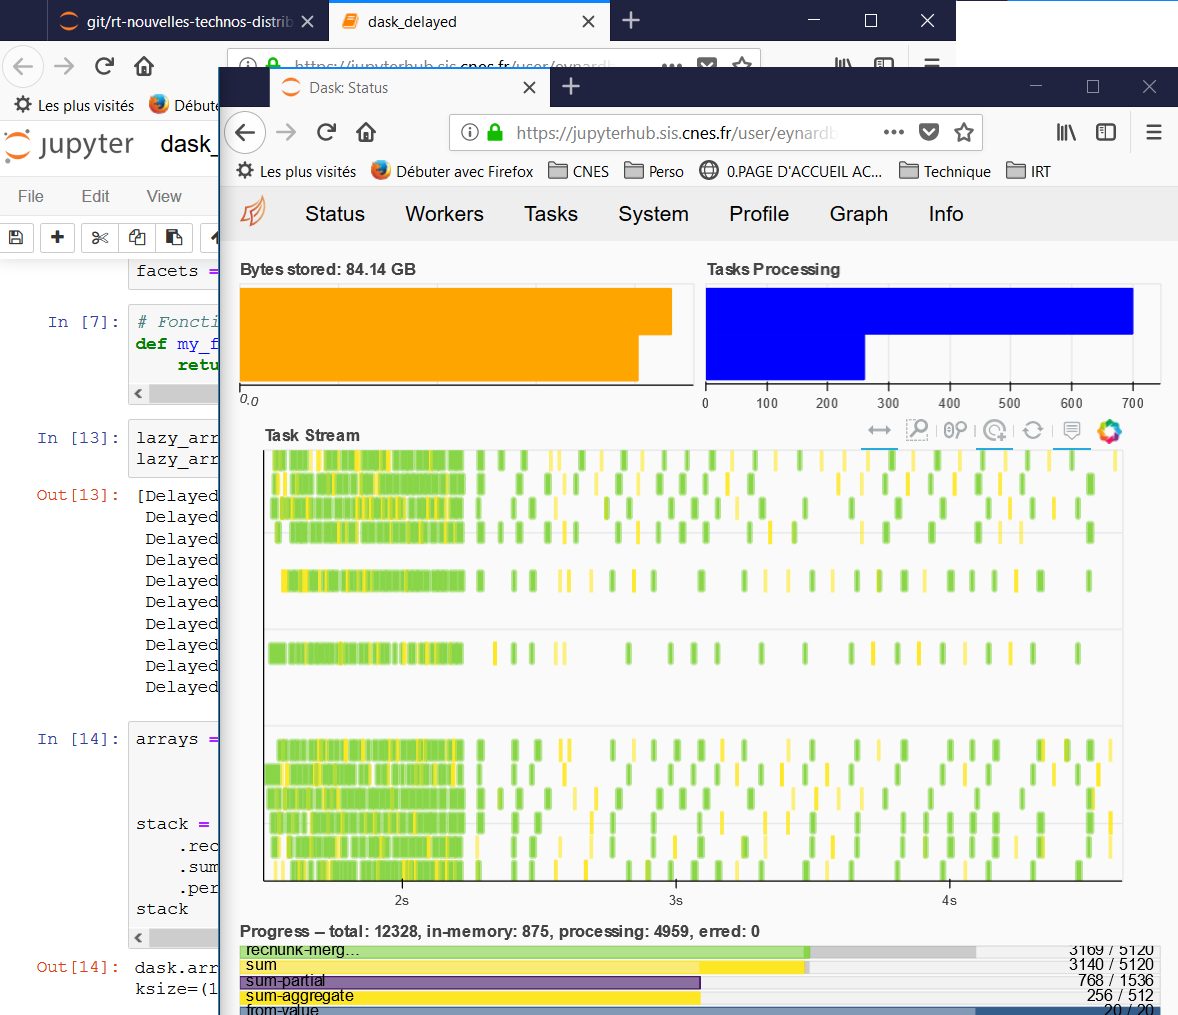
\includegraphics[width=\columnwidth]{dask_jobqueue.png}
  \caption{\label{dask_jobqueue} Computation in Jupyter and Dask dashboard.}
\end{figure}

CNES main processing platform is a modestly sized High Performance Computer named HAL. Its computional resources are: about 8000 Intel cores, 6PB storage using IBM Spectrum Scale technology, some NVidia Volta GPU. It uses PBS Pro jobqueue system to schedule the load on compute nodes and handle user and project resource sharing.

Pangeo platform has recently been deployed on the cluster, which basically means the configuration of two main components: a JupyterHub and Dask through dask-jobqueue (see \ref{dask_jobqueue} for a graphical overview).

JupyterHub has been deployed on a Virtual Machine, which has direct access to HAL cluster through PBS commands. This allows configuring JupyterHub Batchspawner which launch user notebooks using PBS \textit{qsub} command, alongside Wrapspwaner to be able to select adequate system resources for launched notebook.

CNES directly contributes to dask-jobqueue in order to improve its usability on HAL. This Python module deployment (alike Xarray or other domain scientific library) is quite simple as it can be done through conda or pip packaging system. A template configuration is proposed to all HAL users. There is also a few commands documented in order to be able to use the Python environment and thus create Dask clusters from inside Jupyter, some demonstration notebooks have been shared internally.

\subsection{From embarrassingly parallel to more complex workflows with Dask}
\label{ssec:usecase1}

\begin{figure}
  \centering
  \includegraphics[width=0.8\columnwidth]{ep_dask_code.png}
  \caption{\label{ep_dask_code} Embarrassingly parallel workload using Dask's Delayed API.}
\end{figure}

One important use of our cluster is to do batch jobs: apply the same computation or process to several inputs, which can for example be a list of files or a list of parameters. This is usually done with job arrays PBS mechanism. Results are then written into our central storage facility, and a final job will gather them and consolidate them if needed. There are three main drawbacks to this approach:
\begin{itemize}
\item When scaling this mechanism to numerous (say undreds of thousands) and short (under one minute) jobs, this can lead to PBS scheduler contention and slow responsiveness.
\item This often means a lot of bash script and machinery to chain several analysis together, leading to workflows that are hardly readable and difficult to maintain.
\item As results can be really small and are exchanged through a centralized storage system, this also means a lot of I/O load onto the File System and side effects for other users.
\end{itemize}

Pangeo, mainly through Dask, gives an adequate solution to all these problems (see \ref{ep_dask_code} for an example). All the workflow, cluster creation, data management parts are handled from Python code. Reservation to PBS are only done one time using dask-mpi or by bigger blocks using dask-jobqueue for long running worker process. No need to write or exchange data through disk, all data management is done through memory or network with TCP over high-speed networks (i.e. Infiniband). This allows users to analyse the result of a simulation in the same piece of code where we launched it, and eventually gather only the reduced valuable part for later use. The result of all this is elegant and simple Python code, which can scale easily to thousands of cores and does not stress our HPC cluster scheduling components.

\subsection{Interactively simulating remote sensing data through dask array}
\label{ssec:usecase2}

We also used Pangeo to implement the generation of simulated data from a remote sensing satellite. The main idea of the computation is that we need to generate many large two dimensional arrays, each 2 or 4 GB in size, that represent a part of the simulated output, and them sum all of those together. A first implementation was previously done using Python's NumPy and multiprocessing modules, but it was difficult to do the sum in memory, to scale beyond one compute node, and it involved temporary file writing.

Thanks to Jupyter and Dask, we were able to rapidly and interactivly prototype a new algorithm version. Dask solves all of the previous algorithm problems, taking advantage of NumPy array chunking and efficient lazy task execution in graphs for chained operations. One problem remains with our current simple solution: it does not optimize the memory usage, as we need to create all arrays before rechunking and summing them together, but thanks to Pangeo we will fix this soon enough.

\section{Conclusion}
\label{sec:conclusion}

Pangeo is a powerful ecosystem which enables science at scale on Cloud or on premise infrastructure. We encourage every lab, governement agency, or even industry players to take a look at what it provides. The community is open and eager to entrain new users and collaborators.
At CNES, we decided to focus on this tooling for our shared computing infrastructure, and it is already showing its power and its benefit. Ongoing work is focusing on developing more and more use cases with Pangeo to identify where it is most useful, and possible limits to the software stack. A collaboration with the french national institute for marine sciences (Ifremer where the Xarray/Dask environment is already used for science\cite{b9}) on SWOT data valorization is on going and should foster these developments. We are also trying to participate actively in the community and share our vision and needs, helping to steer the common effort in a direction beneficial to CNES researchers.

% To start a new column (but not a new page) and help balance the last-page
% column length use \vfill\pagebreak.
% -------------------------------------------------------------------------
%\vfill
%\pagebreak


% References should be produced using the bibtex program from suitable
% BiBTeX files
% -------------------------------------------------------------------------

\bibliographystyle{plainnat}
\bibliography{myBibFile}

\small

\begin{thebibliography}{00}
\bibitem{b1} Ryan Abernathey, Kevin Paul, Joseph Hamman, Matthew Rocklin, Chiara Lepore, Michaem Tippett, et al. (2017): \href{https://figshare.com/articles/Pangeo_NSF_Earthcube_Proposal/5361094}{Pangeo NSF Earthcube Proposal}.
\bibitem{b2} Mark McInerney, ESDIS Project Deputy Project Manager/Technical: EOSDIS Cloud Evolution\href{https://earthdata.nasa.gov/about/eosdis-cloud-evolution}{NASA EOSDIS web site}.
\bibitem{b3} Ryan Abernathey et al: \href{https://github.com/pangeo-data/pangeo/issues}{Pangeo github project issue tracker}.
\bibitem{b4} Joseph Hamman, Matthew Rocklin, Jim Edwards, Guillaume Eynard-Bontemps, Loïc Estève (2018): \href{https://medium.com/pangeo/dask-jobqueue-d7754e42ca53}{Scalable interactive analysis workflows using dask on HPC Systems}.
\bibitem{b5} Pangeo community: \href{http://pangeo.io/use_cases/index.html}{Pangeo use cases}.
\bibitem{b6} Scott Henderson, Daniel Rothenberg, Matthew Rocklin, Ryan Abernathey, Joseph Hamman, Rich Signell, and Rob Fatland: \href{https://medium.com/pangeo/cloud-native-geoprocessing-of-earth-observation-satellite-data-with-pangeo-997692d91ca2}{Cloud Native Geoprocessing of Earth Observation Satellite Data with Pangeo}.
\bibitem{b7} Ryan Abernathey: \href{https://medium.com/pangeo/step-by-step-guide-to-building-a-big-data-portal-e262af1c2977}{Step-by-Step Guide to Building a Big Data Portal}.
\bibitem{b8} Joseph Hamman, Ryan Abernathey: \href{https://medium.com/pangeo/pangeo-meets-binder-2ea923feb34f}{Pangeo meets Binder}.
\bibitem{b9} S. Fresnay, A. L. Ponte, S. Le Gentil, and J. Le Sommer: Reconstruction of the 3-D Dynamics From Surface Variables in
a High-Resolution Simulation of North Atlantic. \href{https://agupubs.onlinelibrary.wiley.com/doi/abs/10.1002/2017JC013400}{DOI: 10.1002/2017JC013400}.
\end{thebibliography}
\end{document}
